\section{封装与解封流程（参考）}\label{app:seal-unseal-reference}

\subsection{封装流程（参考）}\label{sec:seal-chapter}

\subsubsection{与多文件、目录树的关系}\label{sec:seal-byte-stream-scope}

本章流程的对象是\textbf{按序提交的 Item 载荷}：集成层为每条 Item 产生 \ttf{item_payload}，再调用内容加密并写出 Item。\textbf{每个逻辑文件}（含目录树文件）在密封时仍经同一管道，\textbf{不}因「是否为目录」而变更 Item 形态或密码学步骤（第~\ref{sec:crypto-chapter} 章）。
目录明文结构见第~\ref{sec:directory-tree-chapter} 章；多文件枚举、目录树生成与 Header 中 \ttf{tree_item_index}、\ttf{tree_item_number} 的填写见第~\ref{sec:multi-file-chapter} 章。
本章给出将业务输入写入 \texttt{.aeff} 文件的\textbf{参考流程}。
\textbf{文件格式与可验证约束}以第~\ref{sec:format-chapter}、\ref{sec:crypto-chapter} 章为准；最小不可分单元为 \textbf{Item}，\ttf{item_payload} 的类型与语义须满足第~\ref{sec:item-payload-norms} 节（第~\ref{sec:item-payload-type} 小节）。下文各节为信息性步骤说明，除非某条明确要求校验或布局。

\textbf{子流程（独立说明）：}
\begin{itemize}
  \item 封装上下文（第~\ref{sec:seal-context} 节）；
  \item Item 载荷基本规范（第~\ref{sec:item-payload-norms} 节）；
  \item 滚动摘要累计（第~\ref{sec:rolling-hash} 节）；
  \item Item 写出（第~\ref{sec:item-generation} 节）；
  \item Block 组织与切分（第~\ref{sec:block-split} 节）；
  \item Block 元信息维护（第~\ref{sec:block-meta} 节）；
  \item 收尾落盘（第~\ref{sec:seal-finalize} 节）；
  \item 封装流程总览（第~\ref{sec:seal-total-algorithm} 节，含主循环图与组合调度）。
\end{itemize}
全局一致性见第~\ref{sec:seal-consistency} 节。

\subsection{封装上下文}\label{sec:seal-context}

除按序提交的 \ttf{item_payload} 外，封装侧在调用第~\ref{sec:seal-finalize} 节前 MUST 由集成层提供\textbf{封装上下文}：写入 80 字节 Header 时所需、但\textbf{不能}仅凭 Item 管道内部状态推导的字段与约定。Item 管道\textbf{只消费}封装上下文并写入文件，\textbf{不}规定多文件枚举、目录树明文生成及 \ttf{tree_*} 的推导（见附录~\ref{sec:multi-file-chapter}）。

\textbf{封装上下文（信息性字段表）：}
\begin{itemize}
  \item \ttf{magic_number}、\ttf{version_number}：识别与版本（见第~\ref{sec:header-compat} 节）；
  \item 接收方长期公钥：供第~\ref{sec:item-generation} 节内容加密使用（见第~\ref{sec:curve-keys} 节，应用层提供）；
  \item \ttf{tree_item_index}、\ttf{tree_item_number}：目录树在 Content Region 中的 Item 下标范围（见第~\ref{sec:header-region}、\ref{sec:directory-tree-binding} 节）。无目录树时集成层 MUST 令 \ttf{tree_item_number} $=$ \texttt{0}（\ttf{tree_item_index} 见第~\ref{sec:multi-file-no-tree} 节）；
  \item \textbf{（可选扩展）}实现 MAY 在封装上下文中携带其它应用层元数据；未写入 \texttt{.aeff} Header 的字段不在本标准范围内。
\end{itemize}

\textbf{说明：}
多文件场景下，第~\ref{sec:multi-file-chapter} 章在\textbf{外层}规划 Item 全局顺序并生成目录树 \ttf{item_payload}，在全部 Item 写出完成时 MUST 已确定与内容区一致的 \ttf{tree_item_index}、\ttf{tree_item_number}，再传入第~\ref{sec:seal-finalize} 节。单 Item 流或无目录树时，集成层 MAY 仅提供 \ttf{tree_item_number} $=$ \texttt{0}，其余流程仍按本章执行。

\subsection{Item 载荷基本规范}\label{sec:item-payload-norms}
\label{sec:input-normalization}
本标准以 \textbf{Item} 为 \texttt{.aeff} 内容区最小不可分单元（第~\ref{sec:content-region} 节）。第~\ref{sec:content-encryption}、\ref{sec:decrypt-crypto} 节内容加解密模块、第~\ref{sec:rolling-hash} 节滚动摘要及第~\ref{sec:item-generation} 节 Item 写出，均以本节规定的 \ttf{item_payload} 为\textbf{同一类}输入/输出字节串。

\subsubsection{基本类型（规范性）}\label{sec:item-payload-type}

\ttf{item_payload} 在标准边界上的类型定义如下：

\begin{itemize}
  \item \textbf{类型：}\texttt{VARBYTES}（变长字节串，见第 2 章数据类型），即长度 $L \ge 0$ 的字节序列。$L$ 在\textbf{封装/解封流程与密码学模块}的接口上由集成层提供（内存或 API 参数），用于滚动摘要与内容加解密；\textbf{不是} \texttt{.aeff} 文件里定义的字段类型；
  \item \textbf{与 \ttf{cipher_payload} 的关系：}\texttt{.aeff} 内容区每条 Item 在文件上体现为 \ttf{item_size} 与 \ttf{cipher_payload}（第~\ref{sec:item-record}、\ref{sec:cipher-payload-layout} 节），\textbf{不}直接存放 \ttf{item_payload} 明文字节。封装时，本条 \ttf{item_payload} 经第~\ref{sec:content-encryption} 节写入 \ttf{cipher_payload}；解封时，从 \ttf{cipher_payload} 认证解密得到 \ttf{item_payload}。\ttf{item_size} 仅描述 \ttf{cipher_payload} 长度，与 \ttf{item_payload} 长度无文件内对应字段；
  \item \textbf{语义：}对密码学模块与 \ttf{data_hash} 而言，\ttf{item_payload} 是\textbf{不透明}字节串；标准层不解析其内部为文本、数字、JSON、目录条目等结构；
  \item \textbf{非类型：}\ttf{item_payload} \textbf{不是} Unicode 字符串、数值等宿主类型本身；宿主对象如何变为字节串见下文「与业务载荷的关系」；
  \item \textbf{空载荷：}$L = 0$ 的 \ttf{item_payload} 合法；封装与解封 MUST 对空串及滚动摘要行为保持一致。
\end{itemize}

\subsubsection{与业务载荷的关系}

\begin{itemize}
  \item \ttf{payload} 表示宿主业务对象（如一段文件片段、一条记录）；其类型与切分由应用层决定；
  \item 映射 \ttf{payload} $\leftrightarrow$ \ttf{item_payload}（是否一对一、如何编码）由\textbf{集成层}定义，不属于 \texttt{.aeff} 物理布局；
  \item 解封侧在取得 \ttf{item_payload} 后，由集成层还原 \ttf{payload}；还原规则 MUST 与封装侧对称。
\end{itemize}

\subsubsection{集成层语义约束（规范性）}

\begin{itemize}
  \item 封装与解封 MUST 对 \ttf{item_payload} 采用同一套、且在实现文档中声明的语义（含空串与最大长度策略）；
  \item 每条 Item 对应唯一一条 \ttf{item_payload}；MUST NOT 将多条载荷合并进同一 Item，亦 MUST NOT 将一条 \ttf{item_payload} 拆入多条 Item；
  \item 全部 \ttf{item_payload} MUST 具有确定的\textbf{全局总序}（与内容区 Item 写出顺序一致）；该顺序 MUST 与第~\ref{sec:rolling-hash} 节累计顺序及解封侧输出顺序一致；
  \item 参与滚动摘要的字节串 MUST 与送入第~\ref{sec:content-encryption} 节的 \ttf{item_payload} 逐字节相同。
\end{itemize}

\textbf{说明：}
本标准\textbf{不规定} \ttf{item_payload} 内部的应用层字段布局（与旧版「输入单元」容器无关）。参考实现 \ttf{toNtInput}/\ttf{fromNtInput} 仅为一种集成示例（见附录~\ref{app:ref-impl-symbols}），\textbf{不是}必选格式。

\subsection{滚动摘要累计}\label{sec:rolling-hash}
在封装过程中按 Item 顺序累计全部 \ttf{item_payload} 的滚动摘要，终值写入 Header.\ttf{data_hash}。

\textbf{输入：}
\begin{itemize}
  \item 按 Item 全局顺序的各条 \ttf{item_payload} 完整字节串（见第~\ref{sec:item-payload-norms} 节）；
  \item 初值 $H_0$（当前版本见下文）。
\end{itemize}

\textbf{输出：}
\begin{itemize}
  \item \rollhash 终值 $H_n$（32 字节），封装完成时写入 Header.\ttf{data_hash}（时机见第~\ref{sec:seal-finalize} 节）。
\end{itemize}

\textbf{相关格式：}
Header.\ttf{data_hash} 字段定义见第~\ref{sec:header-region} 节；累计顺序与 Item 写出顺序一致，Item 条数等于参与累计的 \ttf{item_payload} 条数。

\textbf{实施步骤：}
当前版本 (\ttf{version_number = 2}) 规则如下：
\begin{center}
  \texttt{H\_0 = keccak256("Fidelius")} \\
  \texttt{H\_{i+1} = keccak256(H\_i || payload\_i)}
\end{center}
其中第 $i$ 条参与运算的字节串为全局顺序下第 $i$ 个 \ttf{item_payload}（与第~\ref{sec:item-payload-type} 节同型）。记共写出 $N$ 条 Item，终态为 $H_n$。\textbf{\rollhash 终值}\label{sec:rolling-hash-final}定义为 $H_n$；封装完成时 Header.\ttf{data_hash} MUST 等于 $H_n$。

\textbf{说明：}
本节规定递推规则；封装主循环中 $H$ 的初值与更新时机见第~\ref{sec:seal-total-algorithm} 节。每写出一条 Item 前（或同时）应按本节用该 Item 的 \ttf{item_payload} 更新 $H$；终值 $H_n$ 在收尾写入 Header（第~\ref{sec:seal-finalize} 节）。解封侧比对见第~\ref{sec:integrity-check} 节。

\subsection{Item 写出}\label{sec:item-generation}
将一条 \ttf{item_payload} 加密并在内容区追加\textbf{一条} Item 记录。

\textbf{输入：}
\begin{itemize}
  \item 本条 Item 的 \ttf{item_payload}（\texttt{VARBYTES}，见第~\ref{sec:item-payload-norms} 节）；
  \item 接收方长期公钥（应用层提供，见第~\ref{sec:curve-keys} 节）。
\end{itemize}

\textbf{输出：}
\begin{itemize}
  \item 内容区追加的一条 Item：\texttt{[item\_size][cipher\_payload]}（布局见第~\ref{sec:item-record}、\ref{sec:cipher-payload-layout} 节）。
\end{itemize}

\textbf{相关格式：}
一条 \ttf{item_payload} 对应内容区\textbf{一条} Item：\texttt{UINT64(LE) item\_size} 后跟 \ttf{cipher_payload}（见第~\ref{sec:item-record}、\ref{sec:cipher-payload-layout} 节）。

\textbf{实施步骤：}
\begin{enumerate}
  \item 用本条 \ttf{item_payload} 按第~\ref{sec:rolling-hash} 节更新滚动摘要 $H$（更新时机亦可在主循环中单独调度，见第~\ref{sec:seal-total-algorithm} 节）；
  \item 对 \ttf{item_payload} 与接收方长期公钥调用第~\ref{sec:content-encryption} 节，得到 \ttf{item_size} 与 \ttf{cipher_payload}；
  \item 按第~\ref{sec:item-record} 节向内容区追加 \texttt{UINT64(LE) item\_size} 与 \ttf{cipher_payload}。
\end{enumerate}

\textbf{说明：}
组合调度见第~\ref{sec:seal-total-algorithm} 节。向内容区追加顺序见第~\ref{sec:seal-consistency} 节；写出后更新 Header 计数与 Block Info 见第~\ref{sec:block-meta} 节。

\subsection{Block 组织与切分}\label{sec:block-split}
本节说明内容区中的 Block 如何由 Item 构成及何时切分。

\textbf{组织关系说明：}
\begin{itemize}
  \item 内容区由按封装顺序写出的 Item 首尾拼接而成；
  \item 按该顺序将 Item 划分为若干 \textbf{Block}：每个 Block 是其中连续若干条 Item 组成的段，且单个 Block 内 Item 条数 MUST NOT 超过 \ttf{N_block}；各 Block 在 Item 下标与内容区字节偏移上均无隙、无重叠，共同覆盖全部 Item；
  \item 每个 Block 对应 Block Infos 区中的一条 \textbf{Block Info}（32 字节，布局见第~\ref{sec:block-infos} 节）；Header.\ttf{block_number} 为 Block 个数，MUST 等于 Block Infos 区条目数。
\end{itemize}

\textbf{划分规则（当前版本）：}
封装侧按 Item \textbf{写出顺序}维护\textbf{当前 Block}：
\begin{enumerate}
  \item \textbf{首条 Item}：开启第 0 个 Block，该 Block 内仅含本条 Item；
  \item \textbf{并入当前 Block}：若当前 Block 内 Item 条数尚未达到 \ttf{N_block}，本条 Item 并入当前 Block，仅扩展该 Block 的结束下标与结束偏移；
  \item \textbf{切分新建 Block}：若当前 Block 内 Item 条数已达 \ttf{N_block}，则关闭当前 Block 并新建下一 Block，本条 Item 作为新 Block 的首条 Item。
\end{enumerate}
单条 Item MUST 完整地属于一个 Block；MUST NOT 将一条 Item 拆入两个 Block。

\textbf{参考实现：}
当前版本参考实现取 \ttf{N_block = 256}（\ttf{ItemNumPerBlockLimit}，见附录~\ref{app:ref-impl-symbols}）。

\textbf{说明：}
\ttf{N_block} 由封装实现声明，\textbf{不}写入 \texttt{.aeff} 文件；变更且影响互操作时 \ttf{version_number} MUST 递增。
宿主 \textbf{MAY} 将多段业务数据表示为多条 Item（每条独立 \ttf{item_payload}）并写入同一 \texttt{.aeff} 内容区；Block Info 不记录「第几个源文件」，仅索引本文件内 Item 与密文字节。

\subsection{Block 元信息维护}\label{sec:block-meta}
每写出一条 Item 后，封装实现 MUST 按第~\ref{sec:block-split} 节的划分规则，更新 Header.\ttf{item_number} 与内存中的 Block Info 列表，供第~\ref{sec:seal-finalize} 节写入 Block Infos 区。

\textbf{维护对象：}
\begin{itemize}
  \item Header.\ttf{item_number}、Header.\ttf{block_number}；
  \item 长度为 \ttf{block_number} 的 Block Info 列表（每条 32 字节，四字段语义见第~\ref{sec:block-meta-fields} 节）。
\end{itemize}

\textbf{本条 Item 占用字节。} 记刚写出的 Item 其 \ttf{item_size} 字段值为 \ttf{s}（即 \ttf{cipher_payload} 长度），则该 Item 在内容区占用
\[
  L_{\mathrm{item}} = 8 + s
\]
字节（8 字节 \texttt{item\_size} 前缀 + \ttf{cipher_payload}，见第~\ref{sec:item-record} 节）。下文凡写 $L_{\mathrm{item}}$，均指本条 Item 的该占用长度。

\subsubsection{Block Info 字段含义}\label{sec:block-meta-fields}
每条 Block Info 含四个 UINT64 字段，在 \textbf{本 \texttt{.aeff} 文件} 内描述一个 Block 所覆盖的 Item 范围；坐标系均针对该文件的内容区与 Item 序列，\textbf{不}针对业务侧被封装前的源文件。布局见第~\ref{sec:block-infos} 节。

\textbf{Item 下标：\ttf{start_item_index}、\ttf{end_item_index}。}
\begin{itemize}
  \item 含义：本 Block 在内容区 Item \textbf{逻辑序号}上的半开区间 \texttt{[start\_item\_index, end\_item\_index)}。按封装写出顺序，自 \texttt{0} 起为第 0 条 Item、第 1 条 Item……直至 \texttt{item\_number - 1}（与 Header.\ttf{item_number} 一致）。
  \item \ttf{start_item_index}：该 Block 内\textbf{第一条} Item 的下标（\textbf{含}）。
  \item \ttf{end_item_index}：该 Block 内\textbf{最后一条} Item 的下标加 1（\textbf{不含}）；Block 内 Item 条数为 \texttt{end\_item\_index - start\_item\_index}，MUST NOT 大于 \ttf{N_block}；当该值已达 \ttf{N_block} 时，下一条写出的 Item MUST 按第~\ref{sec:block-split} 节开启新 Block；
  \item \textbf{不是}：源明文文件编号、源文件内块号，亦 \textbf{不是} 其它 \texttt{.aeff} 文件中的 Item 下标。
\end{itemize}

\textbf{内容区字节偏移：\ttf{start_file_pos}、\ttf{end_file_pos}。}
\begin{itemize}
  \item 含义：本 Block 在 \texttt{.aeff} 文件 \textbf{Content Region} 内占据的字节半开区间 \texttt{[start\_file\_pos, end\_file\_pos)}。偏移以内容区首字节为 \texttt{0}（内容区在文件最前，故从该文件物理偏移 \texttt{0} 起算）。\textbf{不包含} Block Infos 区与 Header 区（见第~\ref{sec:region-length} 节）。
  \item \ttf{start_file_pos}：该 Block 第一条 Item 的 \texttt{item\_size} 前缀起始处（\textbf{含}）；
  \item \ttf{end_file_pos}：该 Block 末字节的内容区偏移加 \texttt{1}（\textbf{不含}）；Block 在内容区占用 \texttt{end\_file\_pos - start\_file\_pos} 字节。
  \item \textbf{不是}：被封装前原始明文文件（或任意宿主路径下文件）内的字节偏移。字段名 \texttt{file} 指本 \texttt{.aeff} 输出文件的内容区（与参考实现 \texttt{block\_info\_t.start\_file\_pos} 一致），勿与「源文件偏移」混读。
\end{itemize}

\textbf{两对字段的对应关系。}
同一 Block 上，Item 下标区间与内容区字节区间一一对应。
区间内第 \ttf{k} 号 Item（\ttf{start_item_index} $\le$ \ttf{k} $<$ \ttf{end_item_index}）的密文记录 \texttt{[item\_size][cipher\_payload]} 按写出顺序首尾相接，填满 \texttt{[start\_file\_pos, end\_file\_pos)}。
全体 Block Info 在 Item 维度无隙覆盖 \texttt{[0, item\_number)}，在字节维度无隙覆盖 \texttt{[0, content\_size)}。

\textbf{更新规则：}
记刚完成内容区写出、本条 Item 已追加之后：Header.\ttf{item_number} 已为 \ttf{n}（\ttf{n} 从 1 起），刚写入的为第 \ttf{n-1} 号 Item（下标从 0 起）。记 \ttf{cur} 为\textbf{当前 Block} 的 Block Info，即列表中下标 \texttt{block\_number - 1} 的那一条（当 \ttf{block_number > 0} 时）。

\textbf{情形 1：首个 Item}（\ttf{block_number = 0}，\ttf{n = 1}）。新建第 \texttt{0} 条 Block Info，记为 \ttf{cur}：
\begin{itemize}
  \item \ttf{start_item_index} $\leftarrow$ \texttt{0}（不变）；
  \item \ttf{end_item_index} $\leftarrow$ \texttt{1}；
  \item \ttf{start_file_pos} $\leftarrow$ \texttt{0}（不变）；
  \item \ttf{end_file_pos} $\leftarrow$ \texttt{0} $+$ $L_{\mathrm{item}}$；
  \item Header.\ttf{block_number} $\leftarrow$ \texttt{1}。
\end{itemize}

\textbf{情形 2：后续 Item，并入当前 Block}（\ttf{block_number > 0}，且当前 Block 内 Item 条数小于 \ttf{N_block}）。仅更新 \ttf{cur} 的\textbf{结束边界}，起始两字段不变：
\begin{itemize}
  \item \ttf{start_item_index}：不变；
  \item \ttf{end_item_index} $\leftarrow$ \ttf{cur.end_item_index} $+$ \texttt{1}；
  \item \ttf{start_file_pos}：不变；
  \item \ttf{end_file_pos} $\leftarrow$ \ttf{cur.end_file_pos} $+$ $L_{\mathrm{item}}$；
  \item Header.\ttf{block_number}：不变。
\end{itemize}

\textbf{情形 3：后续 Item，新建 Block}（\ttf{block_number > 0}，且当前 Block 内 Item 条数已达 \ttf{N_block}）。令 \ttf{prev} $=$ \ttf{cur}，新建下一条 Block Info（下标为原 \ttf{block_number}）记为 \ttf{cur}，四字段均从前一 Block 的结束处接续：
\begin{itemize}
  \item \ttf{start_item_index} $\leftarrow$ \ttf{prev.end_item_index}；
  \item \ttf{end_item_index} $\leftarrow$ \ttf{prev.end_item_index} $+$ \texttt{1}；
  \item \ttf{start_file_pos} $\leftarrow$ \ttf{prev.end_file_pos}；
  \item \ttf{end_file_pos} $\leftarrow$ \ttf{prev.end_file_pos} $+$ $L_{\mathrm{item}}$；
  \item Header.\ttf{block_number} $\leftarrow$ 原值 $+$ \texttt{1}。
\end{itemize}

\textbf{不变量（每次写出 Item 后 MUST 成立）：}
\begin{itemize}
  \item Header.\ttf{item_number} $=$ 各 Block 的 \texttt{(end\_item\_index -
          start\_item\_index)} 之和；
  \item 各 Block 的 Item 下标区间首尾相接、无重叠，并覆盖 \texttt{[0, item\_number)}；
  \item 各 Block 的 \ttf{start_file_pos}、\ttf{end_file_pos} 首尾相接、无重叠，并覆盖 \texttt{[0, content\_size)}，且 \ttf{content_size} 等于最后一条 Block Info 的 \ttf{end_file_pos}（见第~\ref{sec:region-length} 节）；
  \item 对内容区 Item 的\textbf{全局}下标 $k$（$0 \le k < \texttt{item\_number}$），记第 $k$ 条 Item 在内容区内的起始字节为 $p_k$，占用长度为 $L_{\mathrm{item}}(k)$。则存在唯一的 Block 下标 $t$（$0 \le t < \texttt{block\_number}$），使第 $t$ 条 Block Info 满足
        \[
          \texttt{start\_item\_index} \le k < \texttt{end\_item\_index},
        \]
        且
        \[
          p_k = \texttt{start\_file\_pos}
          + \sum_{j=\texttt{start\_item\_index}}^{k-1} L_{\mathrm{item}}(j)
        \]
        （上式四字段均指第 $t$ 条 Block Info；当 $k$ 等于该条 \texttt{start\_item\_index} 时求和为空）。
\end{itemize}

\textbf{说明：}
情形 2、3 与第~\ref{sec:block-split} 节「划分规则」及 Item 数上限一致；情形 1 对应首条 Item 开启第 0 个 Block。

\subsection{收尾落盘}\label{sec:seal-finalize}
内容区全部 Item 写出后，将 Block Infos 区与 Header 区追加到文件尾部，完成 \texttt{.aeff} 物理布局。

\textbf{输入：}
\begin{itemize}
  \item \textbf{来自 Item 管道：}已写完的内容区及 \ttf{content_size}；\ttf{N} 条 Block Info 取值（\ttf{N = block_number}，由第~\ref{sec:block-meta} 节维护）；滚动摘要终值 $H_n$（第~\ref{sec:rolling-hash-final} 节）；\ttf{item_number}、\ttf{block_number}（由第~\ref{sec:block-meta} 节维护）；
  \item \textbf{来自封装上下文}（第~\ref{sec:seal-context} 节）：\ttf{magic_number}、\ttf{version_number}；\ttf{tree_item_index}、\ttf{tree_item_number}。本节\textbf{不}推导 \ttf{tree_*}，仅按集成层提供的取值写入 Header。
\end{itemize}

\textbf{输出：}
\begin{itemize}
  \item 完整的 \texttt{.aeff} 文件（三区布局见第 4 章）。
\end{itemize}

\textbf{相关格式：}
三区长度见第~\ref{sec:region-length} 节；Block Info、Header 布局见第~\ref{sec:block-infos}、\ref{sec:header-region} 节。
物理写入顺序 MUST 为：内容区 $\rightarrow$ Block Infos 区 $\rightarrow$ Header（第~\ref{sec:seal-consistency} 节）。

\textbf{实施步骤：}
\begin{enumerate}
  \item \textbf{写出 Block Infos 区：}记 \ttf{N = block_number}，自偏移 \ttf{content_size} 起顺序写入 \ttf{N} 条 Block Info（各 32 字节，取值见第~\ref{sec:block-meta} 节）；\ttf{block_infos_size} $= 32 \times N$；
  \item \textbf{写出 Header 区：}紧接其后按第~\ref{sec:header-region} 节写入 80 字节 Header；\ttf{magic_number}、\ttf{version_number}、\ttf{tree_item_index}、\ttf{tree_item_number} 取自封装上下文；\ttf{item_number}、\ttf{block_number} 取自 Item 管道；Header.\ttf{data_hash} MUST 取 $H_n$（\textbf{不得}以 Item 密文另行摘要替代）。
\end{enumerate}
完成后 \ttf{file_size} $=$ \ttf{content_size} $+$ \ttf{block_infos_size} $+$ \texttt{80}。

\textbf{说明：}
进入本节前须已满足：内容区已全部写完；Block Info 与 \rollhash 终值 $H_n$ 已就绪；封装上下文中的 \ttf{tree_*} 已与内容区 Item 布局一致（见第~\ref{sec:seal-total-algorithm}、\ref{sec:multi-file-chapter} 章）。
不在 Header 内存储的应用层伴随元数据（如签名）不在本标准字段约束范围内。

\subsection{封装流程总览}\label{sec:seal-total-algorithm}\label{sec:batch-flush-flow}
本节定义封装侧\textbf{如何组合}前述子流程。各子节仅描述单步职责；本节给出调度变量、主循环参考图及\textbf{按图解读}的实施步骤。

\textbf{变量与状态（仅在本节及图中使用）：}
\begin{itemize}
  \item $H$：滚动摘要状态，初值 $H_0$、终值 $H_n$（递推规则见第~\ref{sec:rolling-hash} 节）；
  \item 待写出 Item 载荷：由集成层按序提供的 \ttf{item_payload}（见第~\ref{sec:item-payload-norms} 节）；
  \item 封装上下文：含 \ttf{magic_number}、\ttf{version_number}、\ttf{tree_item_index}、\ttf{tree_item_number} 等（见第~\ref{sec:seal-context} 节）；多文件时 \ttf{tree_*} 可在主循环前规划、在收尾前最终确认。
\end{itemize}

\textbf{主循环图与子节对应：}
图~\ref{fig:seal-main-flow} 为全量顺序封装的一种参考主流程；图源 \texttt{doc/diagrams/seal-main-flow.mmd}。
\begin{itemize}
  \item 「滚动摘要更新 $H$ / Item 写出」：见第~\ref{sec:rolling-hash}、\ref{sec:item-generation} 节（每条 \ttf{item_payload} 对应一次 Item 写出）；
  \item 「Block 元信息更新」：见第~\ref{sec:block-meta} 节；
  \item 「收尾落盘」：见第~\ref{sec:seal-finalize} 节（传入 Item 管道状态与封装上下文）。
\end{itemize}

\begin{figure}[htbp]
  \centering
  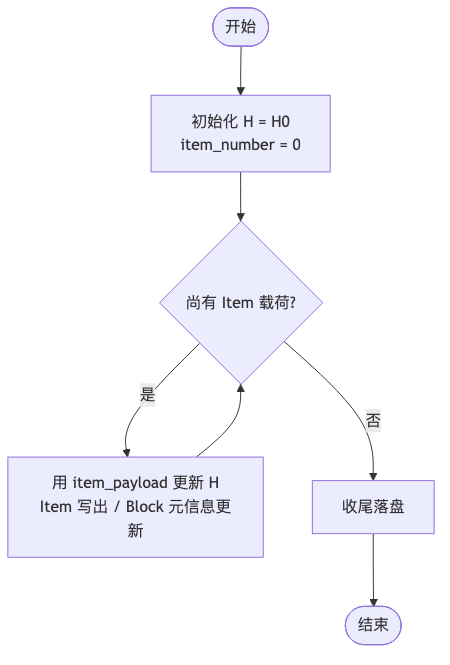
\includegraphics[width=0.85\textwidth]{diagrams/seal-main-flow.png}
  \caption{封装主循环（参考流程；Header.\ttf{tree_*} 由封装上下文提供，见图注及第~\ref{sec:seal-context} 节）}
  \label{fig:seal-main-flow}
\end{figure}

\textbf{实施步骤：}
以下按图~\ref{fig:seal-main-flow} 解读；各步以对应子节为准。
\begin{enumerate}
  \item \textbf{开始与初始化}（图：\texttt{开始}）：准备封装上下文（\ttf{magic_number}、\ttf{version_number} 等）；\ttf{block_number} $= 0$，\ttf{item_number} $= 0$；$H \leftarrow H_0$。无目录树时封装上下文 SHOULD 含 \ttf{tree_item_number} $=$ \texttt{0}。
  \item \textbf{主循环}（图：判断「尚有 Item 载荷」，取\textbf{是}）：集成层提供下一条 \ttf{item_payload}，调用第~\ref{sec:item-generation} 节（含 $H$ 更新与内容区写出），再调用第~\ref{sec:block-meta} 节；返回本步判断。
  \item \textbf{输入结束}（图：判断取\textbf{否}）：确认封装上下文中的 \ttf{tree_item_index}、\ttf{tree_item_number} 与已写 Item 布局一致后，按第~\ref{sec:seal-finalize} 节收尾（\ttf{data_hash} 写入 $H_n$，\ttf{tree_*} 自封装上下文写入 Header）。
\end{enumerate}

\subsection{封装一致性要求}\label{sec:seal-consistency}
\begin{itemize}
  \item 物理写入顺序 MUST 为：内容区 $\rightarrow$ Block Infos 区 $\rightarrow$ Header；
  \item \ttf{item_number} MUST 等于内容区实际 Item 条数；
  \item \ttf{block_number} MUST 等于 Block Infos 区条目数；
  \item 任意 Block Info 的 \ttf{end_file_pos} MUST 不超过 \ttf{content_size}，且相邻 Block 的偏移 SHOULD 首尾相接；
  \item 实现 SHOULD 在封装结束后校验计数与 Header.\ttf{data_hash} 按第~\ref{sec:rolling-hash} 节重算结果一致；
  \item 当 Header.\ttf{tree_item_number} $>$ \texttt{0} 时，\ttf{tree_item_index} 与 \ttf{tree_item_number} MUST 与内容区中目录树 Item 的实际范围一致，且目录树 \ttf{item_payload} 解析后 MUST 满足第~\ref{sec:directory-tree-chapter} 章（规划与校验见第~\ref{sec:multi-file-chapter} 章）。
\end{itemize}

\subsection{解封流程（参考）}\label{sec:unseal-chapter}

\subsection{与多文件、目录树的关系}\label{sec:unseal-byte-stream-scope}

本章规定从 \texttt{.aeff} 按 Item 顺序还原各条 \ttf{item_payload} 并由集成层得到 \ttf{payload}，与密封包内包含几个逻辑文件无关。
将 Item 序列按目录树还原为宿主侧目录结构，属于第~\ref{sec:multi-file-chapter} 章\textbf{整包解封}（目录明文见第~\ref{sec:directory-tree-chapter} 章）；本章仅规定 Item 级认证解密与 \ttf{data_hash} 校验，不重复整包还原步骤。
本章给出从 \texttt{.aeff} 文件按序还原业务载荷的\textbf{参考流程}。
\textbf{文件格式与可验证约束}以第~\ref{sec:format-chapter}、\ref{sec:crypto-chapter} 章为准；解封以 Item 为最小读取与认证单元，\ttf{item_payload} 须满足第~\ref{sec:item-payload-norms} 节且与封装侧同一集成语义。第~\ref{sec:format-chapter} 章「规范性解析流程」中的 MUST 条款在全量顺序解封时与本章一致，本章侧重步骤组合与图示。下文各节为信息性步骤说明，除非某条明确要求校验或布局。

\textbf{子流程（独立说明）：}
\begin{itemize}
  \item Header 获取与校验（第~\ref{sec:unseal-header-model} 节）；
  \item 内容区顺序读取（第~\ref{sec:unseal-item-parse} 节）；
  \item 单条 Item 认证解密（第~\ref{sec:unseal-item-crypto} 节）；
  \item Item 载荷输出与滚动摘要（第~\ref{sec:unseal-item-output} 节）；
  \item 解封流程总览（第~\ref{sec:unseal-total-algorithm} 节，含主循环图、完整性比对与组合调度）；
  \item 进度与可恢复状态（第~\ref{sec:unseal-recoverable} 节，建议性）。
\end{itemize}
上述步骤的\textbf{组合调度}见第~\ref{sec:unseal-total-algorithm} 节；全局一致性见第~\ref{sec:unseal-consistency} 节；失败语义见第~\ref{sec:unseal-errors} 节。

\subsection{Header 获取与校验}\label{sec:unseal-header-model}
从 \texttt{.aeff} 文件尾部取得 Header 记录，校验识别字段并计算三区长度（见第~\ref{sec:read-model} 节）。

\textbf{输入：}
\begin{itemize}
  \item 已打开的 \texttt{.aeff} 文件及 \ttf{file_size}（见第~\ref{sec:region-length} 节）；
  \item \ttf{magic_number}、\ttf{version_number} 的约定取值（见第~\ref{sec:header-current-values} 节）。
\end{itemize}

\textbf{输出：}
\begin{itemize}
  \item \ttf{block_number}、\ttf{item_number}、\ttf{data_hash}；
  \item \ttf{tree_item_index}、\ttf{tree_item_number}（自 Header 解析；Item 级主循环\textbf{不}依赖二者，整包解封见第~\ref{sec:multi-file-chapter} 章）；
  \item \ttf{content_size}、\ttf{block_infos_size}（由 \ttf{file_size} 与 \ttf{block_number} 按第~\ref{sec:region-length} 节算出）。
\end{itemize}

\textbf{相关格式：}
Header 记录布局见第~\ref{sec:header-region} 节；\ttf{data_hash} 字段语义见第~\ref{sec:rolling-hash} 节。

\textbf{实施步骤：}
\begin{enumerate}
  \item 读取文件末尾 80 字节，按第~\ref{sec:header-region} 节解析，得到各 Header 字段；
  \item 将解析得到的 \ttf{magic_number}、\ttf{version_number} 与\textbf{输入}中的约定取值比对；不符时 MUST 终止解封，错误码 SHOULD 为附录 C 中的 \ttf{E_MAGIC_MISMATCH} 或 \ttf{E_VERSION_UNSUPPORTED}；
  \item 令 \ttf{N} $=$ \ttf{block_number}，按第~\ref{sec:region-length} 节计算 \ttf{block_infos_size} 与 \ttf{content_size}；若 \ttf{content_size} 不大于 \texttt{0}，MUST 终止解封，错误码 SHOULD 为附录 C 中的 \ttf{E_FORMAT_TOO_SMALL}（或等价格式错误码）。
\end{enumerate}

\textbf{说明：}
全文件顺序解封\textbf{不必}事先读取 Block Infos 区；块级随机访问须先读 Block Infos 区（见第~\ref{sec:access-capability} 节）。

\subsection{内容区顺序读取}\label{sec:unseal-item-parse}
本节说明全文件顺序解封时，如何从内容区切分出单条 Item 的 \ttf{item_size} 与 \ttf{cipher_payload}。

\textbf{输入：}
\begin{itemize}
  \item \ttf{content_size}、\ttf{item_number}（由第~\ref{sec:unseal-header-model} 节得到）。
\end{itemize}

\textbf{维护的状态：}
与第~\ref{sec:unseal-total-algorithm} 节主循环共享，本节负责在读每条 Item 后更新：
\begin{itemize}
  \item $p$：内容区读指针（相对内容区起点，单位：字节；初值 $p \leftarrow 0$ 见第~\ref{sec:unseal-total-algorithm} 节）；
  \item $n$：已处理 Item 计数（供主循环终止判断及完整性比对；初值 $n \leftarrow 0$ 见同上）。
\end{itemize}

\textbf{输出：}
\begin{itemize}
  \item 本条 Item 的 \ttf{item_size}（记为 $L$）与 \ttf{cipher_payload}。
\end{itemize}

\textbf{相关格式：}
内容区布局见第~\ref{sec:region-length}、\ref{sec:content-region} 节；Item 记录为 \texttt{[item\_size (8B)][cipher\_payload (L B)]}（见第~\ref{sec:item-record}、\ref{sec:cipher-payload-layout} 节）。\textbf{条数不由扫描推断}，以 \ttf{item_number} 为终止条件。本节\textbf{每次调用}读取\textbf{一条} Item。

\textbf{实施步骤：}
\begin{enumerate}
  \item 若 \ttf{content_size} $-$ $p < 8$，MUST 终止本条 Item 读取，错误码 SHOULD 为附录 C 中的 \ttf{E_ITEM_TRUNCATED}；
  \item 自偏移 $p$ 起读取 8 字节，解码为 $L$；若 $L$ 非法（如为 \texttt{0} 或超出实现上限），MUST 终止解封，错误码 SHOULD 为附录 C 中的 \ttf{E_ITEM_SIZE_INVALID}；
  \item 若 \ttf{content_size} $-$ $p < 8 + L$，MUST 终止本条 Item 读取，错误码 SHOULD 为附录 C 中的 \ttf{E_ITEM_TRUNCATED}；
  \item 自偏移 $p + 8$ 起读取 $L$ 字节，得到 \ttf{cipher_payload}；若其布局不满足第~\ref{sec:cipher-payload-layout} 节，MUST 终止解封，错误码 SHOULD 为附录 C 中的 \ttf{E_ITEM_SIZE_INVALID}；
  \item 更新 $p \leftarrow p + 8 + L$、$n \leftarrow n + 1$；当 $n = \ttf{item_number}$ 时，若 $p \ne \ttf{content_size}$，MUST 终止解封（格式错误，如 \ttf{E_ITEM_TRUNCATED} 或实现自定义码）。
\end{enumerate}

\textbf{说明：}
解密与 \ttf{payload} 输出不在本节展开；见第~\ref{sec:unseal-item-crypto}、\ref{sec:unseal-item-output} 节及第~\ref{sec:unseal-total-algorithm} 节。

\subsection{单条 Item 认证解密}\label{sec:unseal-item-crypto}
将一条 Item 的密文载荷还原为 \ttf{item_payload}。

\textbf{输入：}
\begin{itemize}
  \item \ttf{cipher_payload}（由第~\ref{sec:unseal-item-parse} 节读出）；
  \item 接收方长期私钥（应用层提供，见第~\ref{sec:curve-keys} 节）。
\end{itemize}

\textbf{输出：}
\begin{itemize}
  \item \ttf{item_payload}（认证成功后）。
\end{itemize}

\textbf{实施步骤：}
\begin{enumerate}
  \item 对 \ttf{cipher_payload} 与接收方长期私钥调用第~\ref{sec:decrypt-crypto} 节内容解密还原模块；
  \item 若认证失败（第~\ref{sec:auth-failure} 节），MUST 终止解封，MUST NOT 输出 \ttf{item_payload}，错误码 SHOULD 为附录 C 中的 \ttf{E_AEAD_AUTH_FAILED}；
  \item 认证成功时，得到 \ttf{item_payload}。
\end{enumerate}

\textbf{说明：}
算法细节见第~\ref{sec:decrypt-crypto} 节；本章不重复模块内部步骤。

\subsection{Item 载荷输出与滚动摘要}\label{sec:unseal-item-output}\label{sec:unseal-rolling-hash}\label{sec:unseal-batch-output}
将一条 Item 解密得到的 \ttf{item_payload} 用于更新滚动摘要 $H$，并由集成层输出对应的 \ttf{payload}。

\textbf{输入（每次调用）：}
\ttf{item_payload}（由第~\ref{sec:unseal-item-crypto} 节得到）。

\textbf{维护的状态：}
$H$：滚动摘要状态（$H_0$ 见第~\ref{sec:rolling-hash} 节；初值与调度见第~\ref{sec:unseal-total-algorithm} 节）。

\textbf{输出（每次调用）：}
本条 Item 对应的 \ttf{payload}（由集成层从 \ttf{item_payload} 还原）。

\textbf{相关格式：}
\ttf{item_payload} 须满足第~\ref{sec:item-payload-norms} 节；$H$ 递推见第~\ref{sec:rolling-hash}、\ref{sec:rolling-hash-final} 节。

\textbf{实施步骤：}
\begin{enumerate}
  \item 在输出 \ttf{payload} 之前，用本条 \ttf{item_payload} 完整字节串按第~\ref{sec:rolling-hash} 节更新 $H$；
  \item 由集成层将 \ttf{item_payload} 还原为 \ttf{payload} 并输出；语义须与封装侧一致；失败时 MUST 终止解封（格式错误）。
\end{enumerate}

\textbf{说明：}
$H$ 的累计顺序 MUST 与封装侧 Item 顺序一致。完整性比对见第~\ref{sec:unseal-total-algorithm} 节。

\subsection{解封流程总览}\label{sec:unseal-total-algorithm}\label{sec:unseal-main-flow}
本节定义解封侧\textbf{如何组合}前述子流程。各子节仅描述单步职责；本节给出调度变量、主循环参考图及\textbf{按图解读}的实施步骤（含完整性比对）。

\textbf{变量与状态（仅在本节及图中使用）：}
\begin{itemize}
  \item 内容区读指针 $p$、已处理 Item 计数 $n$（由第~\ref{sec:unseal-item-parse} 节维护）；
  \item 滚动摘要状态 $H$（由第~\ref{sec:unseal-item-output} 节维护；$H_0$ 见第~\ref{sec:rolling-hash} 节）；
  \item \ttf{item_number}、\ttf{content_size}、\ttf{data_hash}（由第~\ref{sec:unseal-header-model} 节得到）。
\end{itemize}

\textbf{主循环图与子节对应：}
图~\ref{fig:unseal-main-flow} 为全量顺序解封的一种参考主流程；图源 \texttt{doc/diagrams/unseal-main-flow.mmd}。
图中流程名词与独立子节的对应关系如下（图中\textbf{不}标注章节号；\ttf{data_hash} 等字段语义以正文为准）：
\begin{itemize}
  \item 「读 Header 并校验」「计算 \ttf{content_size}」：见第~\ref{sec:unseal-header-model} 节；图中「初始化 $H = H_0$，$n = 0$」另需 $p \leftarrow 0$（$H_0$ 见第~\ref{sec:rolling-hash} 节）；
  \item 「读 \ttf{item_size} 与 \ttf{cipher_payload}」：见第~\ref{sec:unseal-item-parse} 节（含 $n$ 递增，图中无单独「$n$ 加 1」节点）；
  \item 「认证解密得 Item 载荷」：见第~\ref{sec:unseal-item-crypto} 节；
  \item 「输出 \ttf{payload} 并用 Item 载荷更新 $H$」：见第~\ref{sec:unseal-item-output} 节（须在输出 \ttf{payload} 之前更新 $H$）；
  \item 「$H$ 等于 \ttf{data_hash}」：见下文实施步骤第 3 项（完整性比对）。
\end{itemize}

\begin{figure}[htbp]
  \centering
  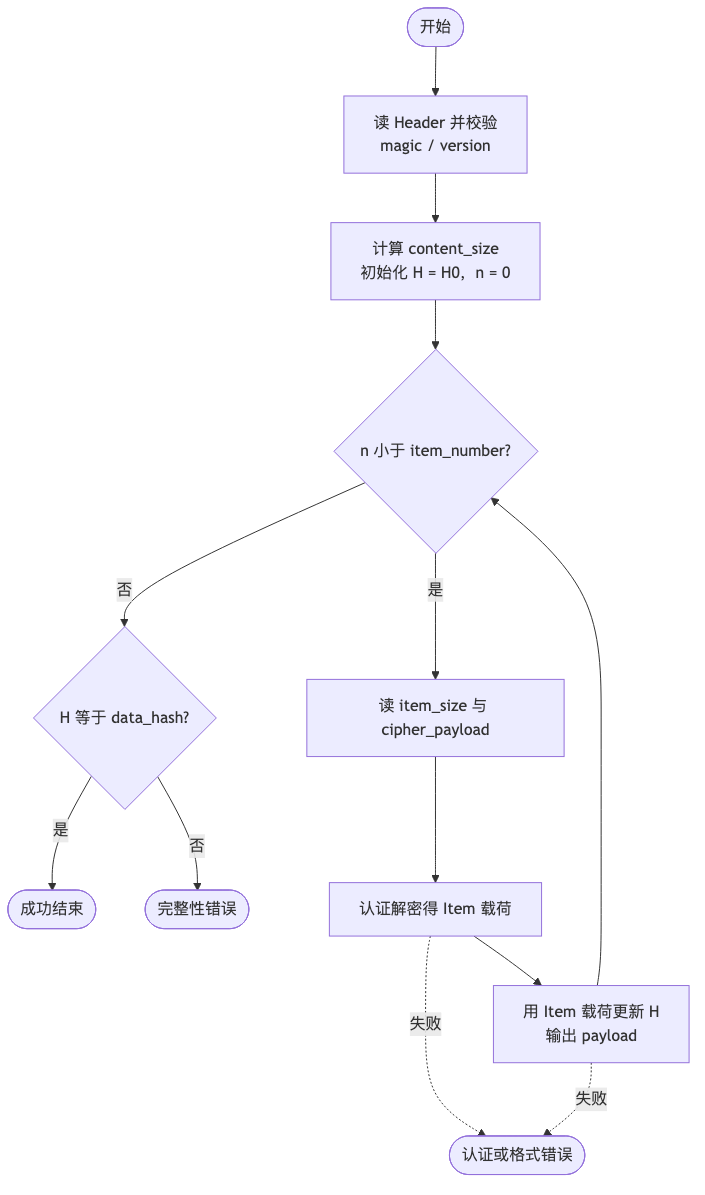
\includegraphics[width=0.85\textwidth]{diagrams/unseal-main-flow.png}
  \caption{解封主循环（参考流程，全量顺序解封）}
  \label{fig:unseal-main-flow}
\end{figure}

\textbf{实施步骤：}
以下按图~\ref{fig:unseal-main-flow} 自上而下解读；各步具体操作以对应子节为准。
\begin{enumerate}
  \item \textbf{开始与 Header}（图：\texttt{开始} $\rightarrow$ 「读 Header 并校验」$\rightarrow$ 「计算 \ttf{content_size} / 初始化」）：按第~\ref{sec:unseal-header-model} 节取得并校验 Header；$H \leftarrow H_0$，$p \leftarrow 0$，$n \leftarrow 0$。
  \item \textbf{主循环}（图：判断 $n$ 小于 \ttf{item_number}，取\textbf{是}）：以当前 $p$、$n$ 调用第~\ref{sec:unseal-item-parse} 节得 \ttf{cipher_payload} 及更新后的 $p$、$n$；调用第~\ref{sec:unseal-item-crypto} 节得 \ttf{item_payload}；以当前 $H$ 调用第~\ref{sec:unseal-item-output} 节输出 \ttf{payload} 并更新 $H$；然后返回本步判断。认证或格式失败时 MUST 终止（图虚线至错误结束）。
  \item \textbf{完整性比对}\label{sec:integrity-check}（图：$n$ 判断取\textbf{否} $\rightarrow$ 「$H$ 等于 \ttf{data_hash}」）：将 $H$ 与 \ttf{data_hash} 逐字节比较；相等则成功结束，不等则 MUST 终止解封，错误码 SHOULD 为附录 C 中的 \ttf{E_INTEGRITY_MISMATCH}，并视已输出的 \ttf{payload} 为不可信；流式输出时 SHOULD 停止下游消费并上报错误。
\end{enumerate}

\subsection{错误处理}\label{sec:unseal-errors}
下列情况 MUST 立即失败，且\textbf{不得}继续输出后续 \ttf{payload}（已输出部分视实现策略可标记为不可信）：
\begin{itemize}
  \item \ttf{magic_number} 或 \ttf{version_number} 校验失败（第~\ref{sec:header-compat} 节）；
  \item \ttf{content_size} 非法，或第~\ref{sec:unseal-item-parse} 节读取 Item 时字节不足或布局非法；
  \item 第~\ref{sec:decrypt-crypto} 节内容解密还原模块认证失败（第~\ref{sec:auth-failure} 节）；
  \item 第~\ref{sec:unseal-item-output} 节 Item 载荷解码或 \ttf{payload} 还原失败；
  \item 第~\ref{sec:unseal-total-algorithm} 节完整性比对中 $H$ 与 \ttf{data_hash} 不一致。
\end{itemize}

\subsection{解封一致性要求}\label{sec:unseal-consistency}
\begin{itemize}
  \item 输出的各段 \ttf{payload} 全局顺序 MUST 与封装侧提交的载荷顺序一致；
  \item 每条 \ttf{payload} MUST 来自经第~\ref{sec:decrypt-crypto} 节认证成功的 \ttf{item_payload}；
  \item 处理完全部 Item 后，$H$ MUST 与 \ttf{data_hash} 一致；
  \item 全文件顺序解封时，实际读取的 Item 条数 MUST 等于 \ttf{item_number}；
  \item 失败时 MUST 符合第~\ref{sec:unseal-errors} 节，不得静默跳过损坏 Item 继续输出。
\end{itemize}

\subsection{进度与可恢复状态（建议）}\label{sec:unseal-recoverable}
支持断点续传或分块交付的实现，在恢复语义下 SHOULD 持久化并可恢复下列状态（名称可因实现而异）：
\begin{itemize}
  \item 已完成处理的 Item 数（对应 $n$）；
  \item 内容区读指针 $p$（含已读 \texttt{item\_size} 前缀与 \ttf{cipher_payload}）；
  \item 滚动摘要状态 $H$（规则 MUST 与第~\ref{sec:rolling-hash} 节一致）；
  \item 已提交给下游的 \ttf{payload} 字节进度；
  \item 已解密但尚未全部交付下游的缓冲（若存在）。
\end{itemize}

\textbf{说明：}
写入端与读取端 MUST 在同一恢复语义下同步推进密文读取偏移与明文提交偏移，避免重复输出或跳写；调度见图~\ref{fig:unseal-main-flow}。
